% ****** Start of file apssamp.tex ******
%
%   This file is part of the APS files in the REVTeX 4.1 distribution.
%   Version 4.1r of REVTeX, August 2010
%
%   Copyright (c) 2009, 2010 The American Physical Society.
%
%   See the REVTeX 4 README file for restrictions and more information.
%
% TeX'ing this file requires that you have AMS-LaTeX 2.0 installed
% as well as the rest of the prerequisites for REVTeX 4.1
%
% See the REVTeX 4 README file
% It also requires running BibTeX. The commands are as follows:
%
%  1)  latex apssamp.tex
%  2)  bibtex apssamp
%  3)  latex apssamp.tex
%  4)  latex apssamp.tex
%
\documentclass[10pt,preprintnumbers,amsmath,amssymb,floatfix,twocolumn,prl]{revtex4-2}
\usepackage[utf8]{inputenc}
\usepackage{amsmath}
\usepackage{mathrsfs}
\usepackage{graphicx}
\usepackage{xspace}
\usepackage[T1]{fontenc}
\usepackage{graphicx}% Include figure files
\usepackage{dcolumn}% Align table columns on decimal point
\usepackage{bm}% bold math
\usepackage{hyperref}
\graphicspath{{./}} 
\usepackage{float}% add hypertext capabilities
%\usepackage[mathlines]{lineno}% Enable numbering of text and display math
%\linenumbers\relax % Commence numbering lines
\usepackage[capitalise]{cleveref}

\begin{document}
\title{A clinical test of the effects of Valerian root on waking hours at night}
\author{Arthur Souza Passos}
\email{a.passos@student.uq.edu.au}
\affiliation{School of Mathematics and Physics, The University of Queensland, QLD 4072, Australia}
\author{Charlie Boardman}
\email{c.boardman1@student.uq.edu.au}
\affiliation{School of Mathematics and Physics, The University of Queensland, QLD 4072, Australia}

\maketitle
%%% WORDCOUNT: 1060 WORDS %%%

\textit{Introduction}: Valerian root is a traditional plant primarily used medically to relieve insomnia and promote sleep \cite{ValerianSource1}. Although a common traditional remedy, medical trials assessing the effectiveness of Valerian root in promoting sleep are limited and have given mixed results \cite{ValerianSource2}. Hence, this study seeks to join this body of literature and help clarify whether Valerian root is an effective at this task. \\

\textit{Methods}: 
We conducted an experimental trial of $n=62$ residents on \emph{the Islands}. We tried to take roughly equal numbers of male and female islanders from a variety of cities across the islands and from many age brackets (20-70 years of age) to distinguish Valerian's effects from age-related, sex-related, and geographical factors which may affect sleep. Each test subject was randomly assigned to take either a 1g tablet of Valerian each night, or be given placebo sugar tablets each night (each with 50\% probability). This gave sample sizes $n_C = 30$ for the control group and $n_V = 32$ Valerian takers. Pills were given between 0.5-2 hours before the islanders' 10:00PM bedtimes (this ensures absoprtion of Valerian into the body \cite{ValerianSource1}) every night for 4 consecutive nights. \\

To measure Valerian's effectiveness in promoting sleep, we analysed if nightly hours of sleep meaningfully decreases in Valerian takers compared to the control group. Waking hours each night were measured from a hypnogram of each test subject’s sleep (within $\pm10$ mins due to graph's limited precision), both before beginning the trial, as well after 1-4 nights afterward. This limited number of nights prevents our result from being affected by the development of tolerances to Valerian's effects. \\

%%% NOTE: C and V are used as indices in the below working, not as powers %%%
Our test subjects' sleep habits over the trial may be influenced by their Valerian consumption, and external factors such as their age, personal health, and environment. Assuming linearity in the number of nights $t$ since trials began, the mean waking hours $y^C$ for the control group and $y^V$ for the Valerian takers will be:
$$y^C = \beta_0^C + \beta_1^C t, \qquad y^V = \beta_0^V + \beta_1^V t$$
For some parameters $\beta_0^C, \beta_0^V$ denoting baseline average waking hours before the trial began, and $\beta_1^C, \beta_1^V$ representing the rate per day of waking hour increases. If each test subject's waking time is independent of the others', and our data is normally distributed around our two lines with a variance independent of $t$, we can estimate these parameters and their standard deviations $\sigma_0^C, \sigma_1^C, \sigma_0^V, \sigma_1^V$ from a linear regression model. \\

If both the control and Valerian taker groups are representative of the islands' population (and hence the external factors they are under), the nightly changes $\beta_1^C, \beta_1^V$ should have no difference besides those due to Valerian's effects. Hence, we test the hypotheses:
$$H_0: \beta_1^C = \beta_1^V, \qquad H_1: \beta_1^C > \beta_1^V$$
Where the null hypothesis $H_0$ corresponds to Valerian having no effect on waking hours at night, and the alternative hypothesis $H_1$ corresponds to Valerian producing a statistically significant reduction in waking hours each night relative to the control group. Our estimates of $\beta_1^C, \beta_1^V$ should be $T$-distrubuted under our assumptions, with degrees of freedom $5n_C - 2, 5n_V - 2$ (for $n_V$ or $n_C$ subjects tested over 5 nights) respectively. Hence, assuming our null hypothesis, we expect the below to be $t_\text{df}$-distributed:
$$T = \frac{\beta_1^C - \beta_1^V}{\sqrt{\frac{(\sigma_1^C)^2}{5n_C} + \frac{(\sigma_1^V)^2}{5n_V}}}$$
Where the degrees of freedom (df) is given by Welch's approximation:
$$\text{df} = \frac{\left(\frac{(\sigma_1^C)^2}{5n_C} + \frac{(\sigma_1^V)^2}{5n_V}\right)^2}{\frac{(\sigma_1^C)^4}{(5n_C)^2 (5n_C - 2)} + \frac{(\sigma_1^V)^4}{(5n_V)^2 (5n_V - 2)}}$$
We then compute the probability of our data being more extreme than predicted from our $T$ value assuming $H_0$ as $p = \mathbb{P}(t_{df} \geq T)$ and evaluate our hypotheses against a standard 95\% confidence criterion. \\

\textit{Ethics}: Consent was obtained from all islanders we tested on. Since Valerian root may be a sedative (and hence interact with alcohol \cite{ValerianSource1}), all test subjects were instructed to reduce alcohol consumption during the trial. As little is known of valerian's effects on pregnancies \cite{ValerianSource2}, pregnant women were excluded from our study. \\

\textit{Results}: Linear regression models were fitted to both the control and valerian groups' data to estimate the baseline waking hours per night ($\beta_0^C, \beta_0^V$) and the average rate of change in waking hours per night ($\beta_1^C, \beta_1^V$). For the control group the model was determined by:
$$
y^c = 133.9 - 2.92 t
$$
with the slope estimate: $\beta_1^c = - 2.92$ having a standard error of 1.80.
The model for the valerian data was given by: 
$$
y^V = 118.1 - 3.56 t
$$
with the slope estimate: $\beta_1^v = - 3.56$ having a standard error of 1.51.
Both slope estimates were slightly negative (discussion) indicating a minor decrease in waking minutes per night over the course of the trial for both groups. The valerian group indicated a steeper decline in waking minutes per night, however using a welch test this difference in slope was found to be statistically insignificant. 
\begin{figure}[H]
\centering
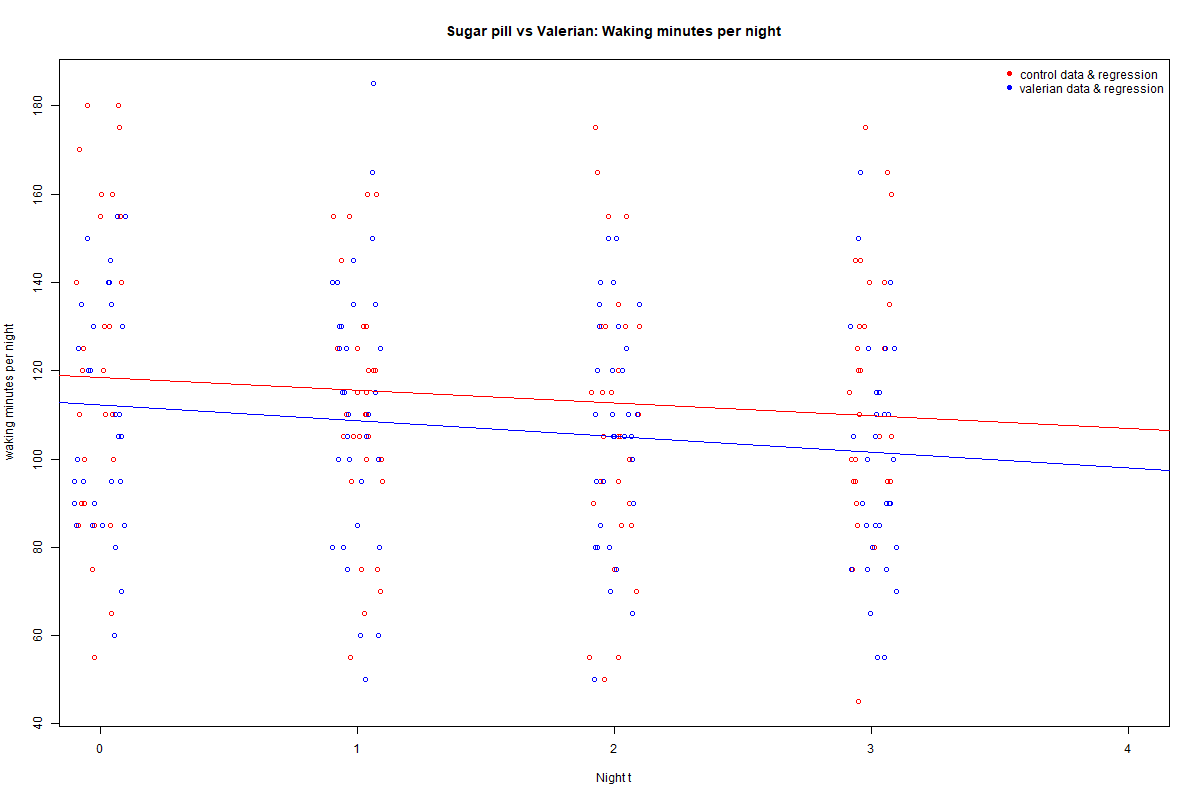
\includegraphics[width=0.95\linewidth]{linear_reg.png}
\caption{Waking minutes per night for Control (red) and Valerian (blue) groups with fitted regression lines. NOTE: discreet time values are jittered for clear distinction of data points.}
\end{figure}
Using these slope estimates and their standard errors, we computed the test statistic $T$ and degrees of freedom $df$ using Welch's t-test, giving: $T = 0.27$ and $df \approx 294$. From this the p-value was calculated as $P = 0.39$
Diagnostic plots, including QQ plots and residuals vs fitted value plots, were created for both linear models in order to asses the validity of the linear regression assumptions. These plots are displayed below. 
\begin{figure}[H]
\centering
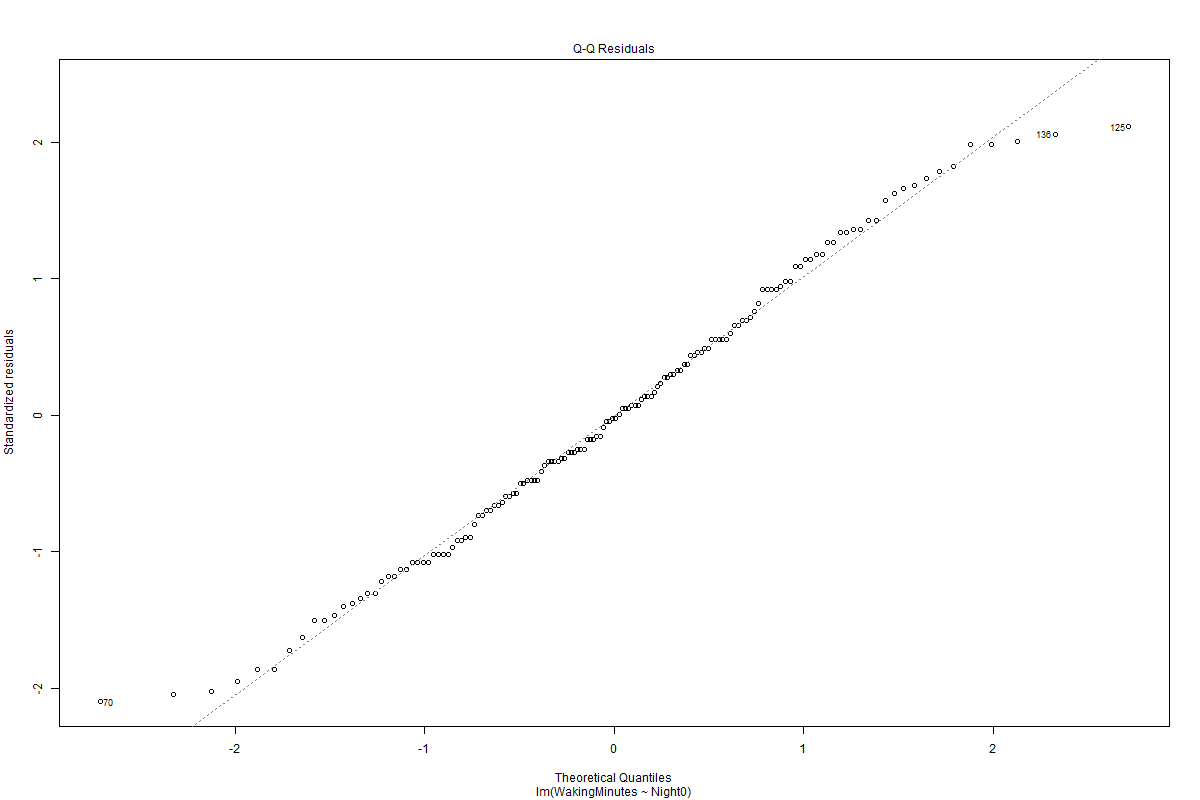
\includegraphics[width=0.95\linewidth]{QQ_control.png}
\caption{QQ plot of standardized residuals for the control group. The residuals align closely with the theoretical quantiles, suggesting normality in the model.}
\end{figure}

\begin{figure}[H]
\centering
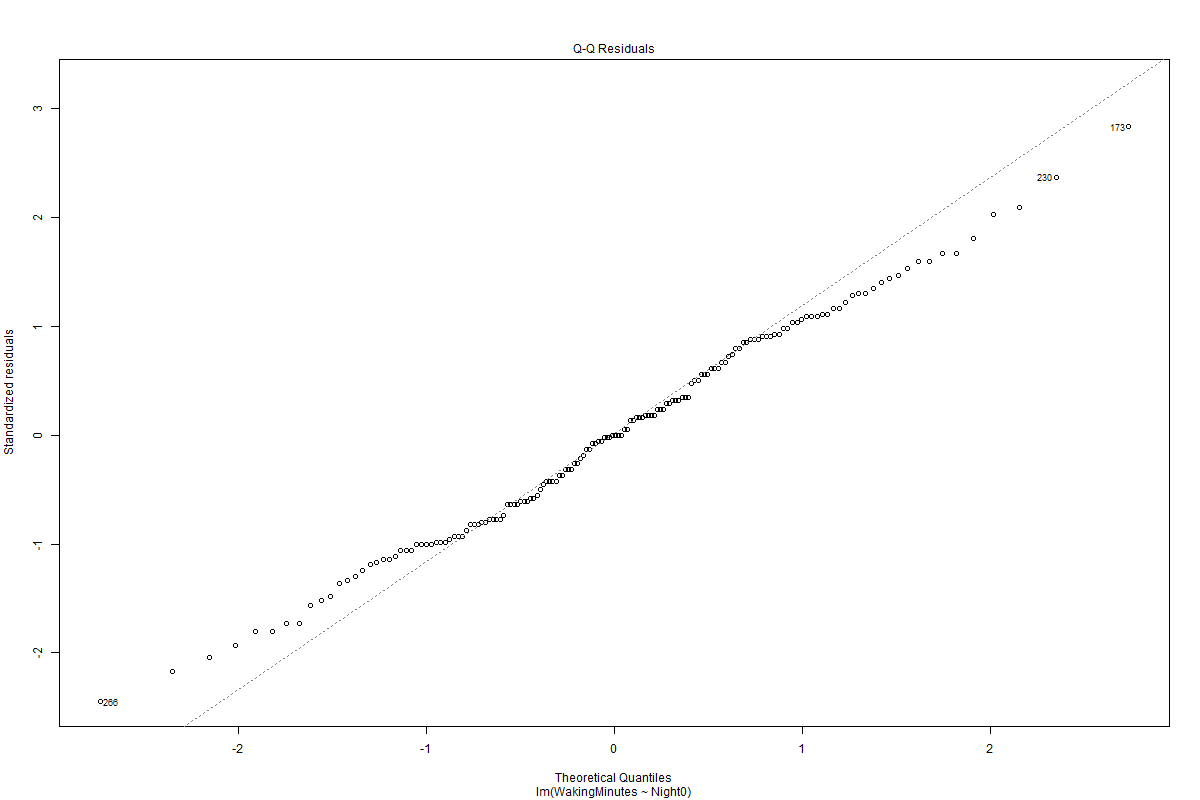
\includegraphics[width=0.95\linewidth]{QQ_valerian.png}
\caption{QQ plot of standardized residuals for the valerian group. The residuals aliign with the theoretical normal around 0, with slight deviations at either end.}
\end{figure}

\begin{figure}[H]
\centering
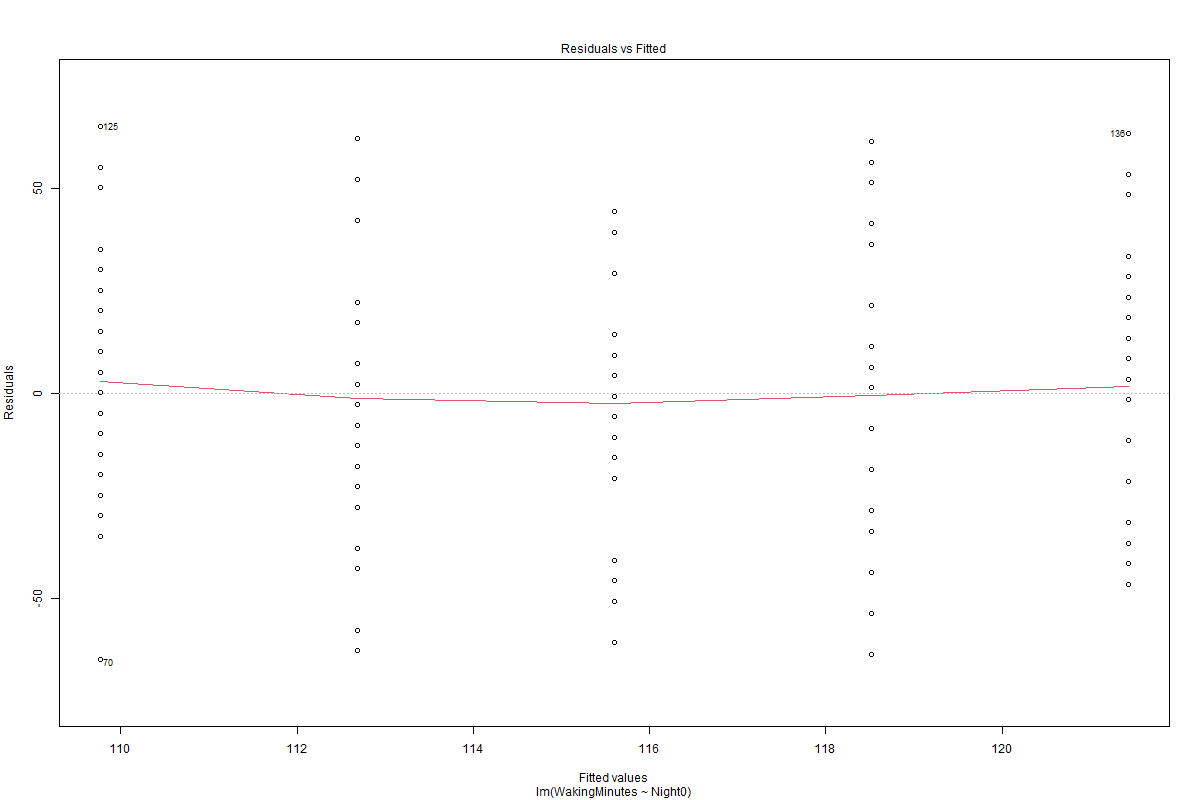
\includegraphics[width=0.95\linewidth]{residual_fitted_control.png}
\caption{Residuals versus fitted values for the control group. Residuals are evenly scattered around zero with no significant curvature, indicating constant variance in the fitted model.}
\end{figure}

\begin{figure}[H]
\centering
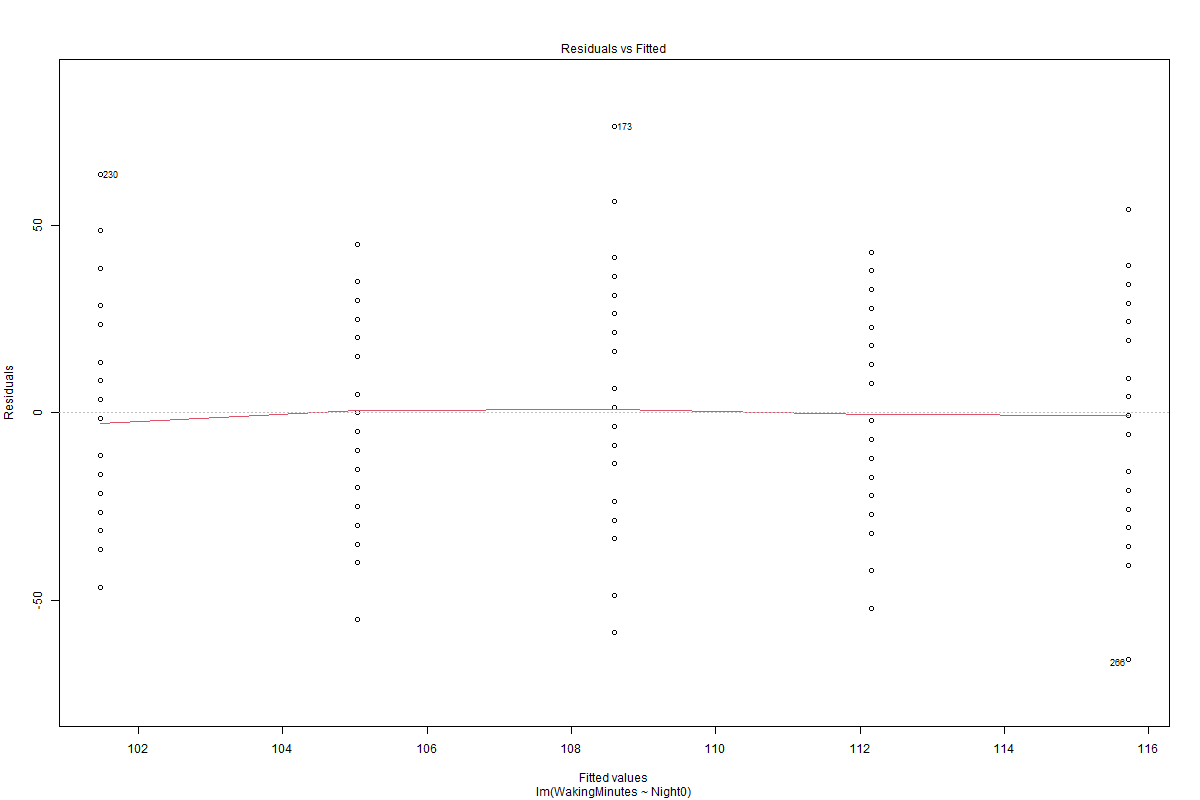
\includegraphics[width=0.95\linewidth]{residual_fitted_valerian.png}
\caption{Residuals versus fitted values for the Valerian group. Residuals show a random distribution without clear patterns, indicating constant variance in the fitted model.}
\end{figure}

All graphs indicate that the assumptions of the linear regression model are satisfied. The larger than expected extreme residuals of the QQ plot for the valerian model may indicate a small number of outliers were included in the group.\\

\textit{Discussion and Conclusion}: Data collected from both groups displayed a minimal decrease in waking minutes per night over the course of the trial, with the valerian group showing a slightly steeper decrease. This decrease can be attributed to a variety of factors, including a difference in participant demographics, environmental variation such as a higher proportion of valerian takers coming from naturally darker or quieter locations. 
Research with a larger sample size and stricter control of external factors is needed to further investigate the effects of valerian root on sleep quality. Furthermore, the decision to measure sleep quality based on waking minutes per night may not be the most effective approach. Future studies could instead focus on other measurements such as time taken to fall asleep or time spent in different sleep stages.
The P-value of $P = 0.39$ leads to the rejection of our alternative hypothesis $H_1: \beta_1^C > \beta_1^V$ at a 95\% confidence interval. The rejection of $H_1$ indicates that there is insufficient evidence to suggest that there is a significant corelation between the use of valerian root and a reduction in waking minutes per night



\bibliographystyle{apa}
\bibliography{ResearchProjectReportBibliography}

\end{document}
